% Аспекты внешней среды
% 8. Какие факторы внешней среды Вы учитываете при анализе функционирования системы?
% 9. Какой информацией о факторах внешней среды Вы располагаете (детерминированные, случайные, интервально неопределенные, активное противодействие «противника» или конкурента)?
% 10. Какие показатели эффективности системы в целом и ее подсистем Вы рассматриваете?
% 11. Как в этих показателях учитывается информация о внешней среде?

Внешними факторами для системы являются исходный объем требований ТЗ $R^*$ и требования текущего заказчика $R^{*}_{n}$. При формировании поставки, в нее включается реализация требования непотребных заказчику $R^{*}_{un}$ в связи с наличием в проекте функциональных зависимостей. Поставляемый объем требований $R^{*}_{d} = R^{*}_{n} \cup R^{*}_{un}$. От $|R^{*}_{un}|$ зависит коэффициент бесполезности $K_{f}$. Этим коэффициентом характеризуется степень холостой работы подразделений постпродажного обслуживания сформированной поставки компанией производителем. $K_{f} = |R^{*}_{un}| / |R^{*}_{d}|$.

Например, заказчик запросил 10 требований, а поставлен был функционал, реализующий 15. 5 требований он не оплатил, но осуществлять их поддержку все равно необходимо. В данном случае $K_{f} = 5 / 15 = 1/3$. Почти 33\% работы персонала по постпродажному обслуживанию поставки программного средства заказчиком не оплачена.

Графическая интерпритация приведенных множеств приведена на рисунке \ref{fig:life_circle}.

\begin{figure}[H]
    \centering
    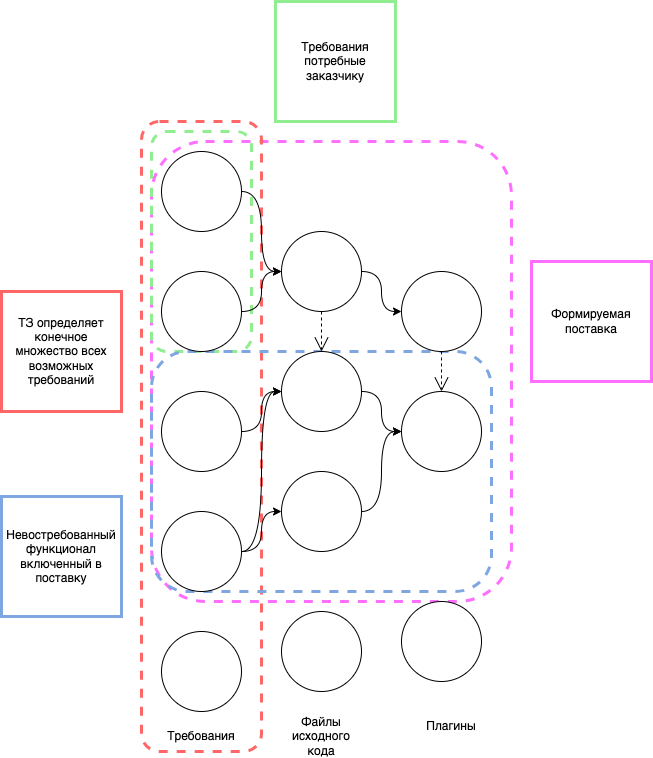
\includegraphics[width=1\textwidth]{life_circle}
    \caption{Формирование поставки по потребным заказчику требованиям}
    \label{fig:life_circle}
\end{figure}

С другой стороны, существуют затраты на разработку и поддержку программного средства. Чем больше его кодовая база $V_{c}$, тем дороже его разработка, отладка и управление его конфигурацией.

Подытоживая, от показателей $K_{f}$ и $V_{c}$ зависит рентабельность программного средства, а значит и конкурентоспособность бизнеса.